% !TeX program = xelatex
% !TeX encoding = UTF-8
\documentclass[UTF8,a4paper,12pt,fontset=fandol]{ctexart}

\usepackage{amsmath,amssymb,bm,mathtools}
\usepackage{geometry}
\usepackage{graphicx}
\usepackage{float}
\usepackage{xcolor}
\usepackage{listings}
\usepackage{enumitem}
\usepackage{booktabs,longtable,array}
\usepackage[hidelinks,unicode]{hyperref}
\usepackage{bookmark}

\geometry{top=2.54cm,bottom=2.54cm,left=3.0cm,right=2.6cm}
\setlength{\parindent}{2em}
\setlength{\parskip}{0.35em}
\linespread{1.35}
\graphicspath{{figures/}}
\hypersetup{
  pdftitle={质点轨迹重构算法专利技术交底书},
  pdfauthor={},
  pdfsubject={质点轨迹重构算法}
}

\lstdefinestyle{patentpseudo}{
  basicstyle=\ttfamily\small,
  columns=fullflexible,
  keepspaces=true,
  breaklines=true,
  breakatwhitespace=false,
  frame=single,
  rulecolor=\color{black!25},
  backgroundcolor=\color{black!2},
  showstringspaces=false
}

\title{质点轨迹重构算法专利技术交底书}
\author{}
\date{}

\begin{document}
\pagestyle{plain}
\maketitle

\section{发明名称}

一种基于时间重分配的质点轨迹重构方法。

\section{技术领域}

本发明涉及机器人运动规划、无人系统轨迹规划、数控运动控制及计算机辅助轨迹生成技术领域，特别涉及一种在给定空间航点和受限轴向加速度条件下，通过重新分配各航段通过时间和航点速度，生成累计运动时间较短的三维质点轨迹的方法。

本发明所处理的对象可以抽象为具有三维位置、三维速度和三维加速度状态的质点。该质点可以代表无人飞行器的平动参考点、移动机器人或自动驾驶车辆在局部坐标系中的规划参考点、机械执行机构的末端参考点、搬运设备的载荷参考点，也可以代表其他满足二阶积分运动近似的受控对象。本发明生成的是位置、速度和加速度层面的参考轨迹，不以某一种具体飞行器结构或编程语言为前提。

本发明中的“时间重分配”是指：在保留有序航点通过约束以及给定起始、终止运动状态的基础上，不直接沿用输入参考路径原有的时间戳和速度大小，而是重新确定各中间航点处的候选速度、相邻航点之间的公共持续时间、各坐标轴的加速度阶段及其切换时刻，由此形成新的时间参数化轨迹。本发明并不要求输入对象已经具有完整时间信息，输入可以是纯几何航点序列，也可以是从任意参考轨迹中提取的航点及局部运动方向。

\section{背景技术}

对无人飞行器、移动机器人和高速执行机构而言，路径与轨迹具有不同含义。路径主要描述从起点到终点所经过的空间位置或几何曲线，而轨迹还需要描述在什么时刻到达什么位置，并进一步给出速度、加速度乃至更高阶运动状态。一个几何上可行的路径，如果时间参数化过于激进，可能超出执行机构的加速度能力；如果时间参数化过于保守，则会造成完成任务所需时间过长，不能充分利用系统的动态性能。

现有局部路径规划或轨迹优化方法通常同时考虑障碍物、平滑性和动力学可行性。为了降低非线性优化难度，一类方法先生成几何可行路径，再执行时间参数化；另一类方法直接优化多项式或样条的控制点和分段时间。直接联合优化的位置变量、时间变量和高阶导数变量数量较多，容易受到初值影响，并且在需要快速重规划时具有较高计算负担。先确定空间路径再分配时间的方法能够分离几何规划与动态调度，但仍需解决如何选择航点速度、如何计算相邻航点之间的最短可行转移时间，以及如何保证三维坐标同时到达下一航点的问题。

常见的简单时间分配方式按照航段长度与预设巡航速度的比值设置航段时间，或者按照全部航段长度的比例缩放原始时间。这些方法容易实现，但通常没有显式利用各坐标轴允许的正、负加速度。当路径转弯方向发生变化时，只依据欧氏距离分配时间不能准确描述三个速度分量的调整难度。例如，某一航段在x轴上位移较大且需要显著改变x轴速度，而在y轴和z轴上位移较小，三个坐标轴实际所需的动态转移时间并不相同。若各轴独立执行，则会出现到达时刻不一致；若简单采用统一的保守缩放，则会损失可利用的动态性能。

另一类方法在离散路径点上求取路径参数速度，并通过前向、后向积分或者凸优化满足速度和加速度约束。这类方法适合沿给定连续曲线进行严格路径参数化，但需要明确曲线的一阶、二阶几何导数，并将执行器约束转换到路径参数域。在输入仅为稀疏航点和局部方向信息时，路径导数可能不完整；同时，对在线规划而言，连续优化或大规模约束求解的计算量也可能较高。

对于二阶积分质点，如果一维起末位置、起末速度及加速度上下界已知，则采用两个恒定加速度阶段能够解析计算候选转移时间。其基本形式是先使用一个方向的加速度，再切换为相反方向的加速度，以便同时满足末端位置与末端速度。不过，将该思想直接扩展到三维仍存在至少三个困难：第一，各坐标轴的独立最短时间一般不同；第二，为了让质点准确通过三维航点，需要三个坐标轴采用同一航段持续时间；第三，中间航点速度既影响前一航段又影响后一航段，仅逐段贪心选择当前最快速度可能导致总时间并非最小。

对中间航点速度进行连续优化会形成含多个速度分量、阶段时间和切换时刻的耦合问题。若完全独立采样三个速度分量，候选数量会随维数呈乘法增长，并可能产生与参考路径局部走向明显不符的速度方向。若仅把输入轨迹的原速度直接作为航点速度，则无法发挥重新分配时间的作用。因此，需要一种既能利用参考运动方向降低搜索维度，又能在多个航段之间联合选择速度幅值的方法。

此外，实际运动系统通常要求轨迹生成模块直接输出按统一周期排列的位置、速度和加速度参考值。单纯得到每段总时间或航点速度尚不足以形成可执行轨迹。还需要恢复每个轴的加速度顺序、加速度大小、切换时刻、切换速度和切换位置，并在坐标轴之间保持时间对齐。对于某一轴位移为零、二次方程退化、候选转移无实数根或者同步缩放因子超过允许范围等情况，也需要提供明确处理规则。

\section{现有技术存在的问题}

从输入信息与求解变量的关系看，航点位置只规定必须经过的空间状态，不能唯一决定到达时间和通过速度。同一组航点可以对应多条位置与速度连续的轨迹，其中有些轨迹在某个方向上先制动再加速，有些轨迹则先加速再制动。若时间分配没有同时使用端点速度，便无法区分这些动态过程，也无法保证给定终端速度。对于重复位置或者很短的航段，这种区别尤为明显：几何长度可能接近零，而速度改变仍需要非零时间。

从航段之间的联系看，中间航点并非若干互不相关问题的分界。选择较大的通过速度，可能降低驶入航段的时间，却增加驶出航段的制动或换向时间；选择较小的通过速度，则可能产生相反结果。因此，先单独求出每段的最快运动再拼接，通常不能同时满足共享速度条件。问题需要显式记录航点速度，使前后两段对同一边界状态达成一致，再比较整个序列的累计时间。

从多轴同步的角度看，能够在某个时间之前到达目标状态，与能够在指定时间恰好到达目标状态，是不同的约束。尤其当端点速度不为零时，任意增加持续时间并不等于在终点静止等待；等待会改变端点速度或者要求新增运动阶段。同步过程需要同时求解时间、切换时刻和实际加速度，而不能只用最大轴向时间替代这一步骤。一个合格的航段代价应当伴随能够实现该代价的运动参数。

从结果表达看，离散位置点本身不能充分证明加速度约束和端点速度约束成立。采样间隔越大，隐藏在采样点之间的加速度切换越容易被忽略。因而应将解析运动参数作为基本结果，采样点作为由该结果得到的输出形式；这样即使输出周期改变，也仍可用同一组参数检查端点、阶段时长与加速度边界。上述输入、同步、跨段耦合和解析输出问题共同构成本发明处理的技术问题。

因此，现有技术至少存在如下不足：缺少一种面向有序三维航点的轻量化时间重分配方法，能够把中间航点速度选择、受限加速度航段时间计算和三轴同步统一到同一求解框架中；难以在不进行高维连续联合优化的条件下，对多个航段的累计时间进行整体选择；以及难以将速度搜索结果直接、解析地恢复为位置、速度和加速度轨迹。

针对上述问题，有必要提供一种独立于上游路径生成方式的质点轨迹生成方法。该方法应当能够接收任意来源的航点及参考方向，把多个航点处的速度幅值选择转化为结构明确的离散搜索问题，以轴向受限加速度模型计算航段代价，并通过公共时间同步和解析重构得到统一时间轴上的三维质点轨迹。

\section{发明目的}

本发明的首要目的在于提供一种基于时间重分配的质点时间最优轨迹生成方法，在不依赖特定上游路径规划器、不要求输入完整连续曲线参数方程的情况下，根据有序航点、参考运动方向和轴向加速度边界，联合确定中间航点速度和各航段持续时间，从而在规定离散候选可行域内减小质点通过全部航点所需的累计时间。

本发明的另一目的在于把三维质点的受限加速度转移分解为三个低维的一维分段恒加速度问题。三个独立轴向最短时间的最大值仅作为公共时间下界；通过验证各轴在同一持续时间下的切换时刻、实际加速度和端点状态，取得三轴可同步时间集合交集中的最小值，从而避免把“单轴所需时间不超过某值”误当成“该轴必能恰好在该时间完成”。

本发明的又一目的在于把多个中间航点处相互耦合的速度选择问题表示为分层速度图上的累计时间最短路径问题。每一中间航点只需沿参考运动方向设置多个候选速度幅值，因而相对于分别枚举三个速度分量能够显著减少候选组合数量，同时通过跨航段累计代价避免单航段贪心选择。

本发明还旨在提供一种从搜索结果到可执行参考轨迹的确定性恢复方式。通过保存最优节点的前驱关系以及每个航段的两阶段时间、加速度方向、缩放因子和切换状态，能够按统一采样周期直接生成质点位置、速度和加速度序列，便于向后级运动控制器提供参考状态。

\section{技术方案总体说明}

为实现上述目的，本发明把整个求解过程划分为航点数据预处理、候选速度生成、分层速度图构建、轴向转移时间求解、三轴时间同步、累计时间最短路径搜索、最优节点链回溯以及质点轨迹解析重构八个环节。各环节只通过明确的数学量传递数据，能够作为独立软件程序运行，也能够嵌入更大的运动规划系统。

基于上述方法，本发明还提供一种质点时间最优轨迹生成系统。该系统包括输入处理模块、候选速度生成模块、分层图构建模块、轴向转移求解模块、时间同步模块、路径搜索模块和轨迹重构模块。

本方法能够独立使用。输入端只需要有序航点位置、用于构造中间速度候选的参考方向、起始速度、终端速度、候选幅值和轴向加速度区间；这些量可以由人工设定、几何路径离散、历史轨迹抽取或任何外部规划过程提供。算法不调用也不依赖某一特定前端规划器，外部规划过程的名称、数据结构和优化目标均不是本发明必要特征。

输出端给出统一时间轴上的质点位置、速度和加速度，以及必要时给出航点速度、各航段公共持续时间与切换参数。输出不包含姿态、角速度、推力或控制器命令。若下游系统需要这些量，应根据具体对象模型另行变换，并重新验证其自身约束。该分工保持本方法作为“质点轨迹重构算法”的独立边界。

每次求解对应一组固定输入。若任一航点、参考方向、端点速度、候选集合或加速度边界变化，应重新计算受影响的候选边并重新执行动态规划；仅沿上一结果路径局部更新而不比较其他候选，不能保证新输入下仍为有限图内最优。缓存未变化边仅是计算复用，不改变数学结果。

当所有输入航点及候选集合给定后，算法可能有两类正常输出：存在终止节点可达路径时返回最优重构轨迹；不存在时明确返回规定候选集合和控制族内不可行。不可行不等于任意质点轨迹都不存在，可能只是候选速度过少或共同缩放两阶段控制族过窄。扩大候选集合或控制族会形成新的优化问题，应重新评价其最优性范围。

输入处理模块可以接收航点位置矩阵、参考方向矩阵、当前状态和约束参数，并执行维数、有限数值、航点数量和上下界关系检查。若航点数小于二、坐标包含非有限值、任一轴不满足加速度下界严格小于零且上界严格大于零，或者候选集合无有效元素，则输出明确错误状态。近零参考方向按候选构建章节的规则处理。输入处理模块不需要了解航点由何种前端算法生成。

候选速度生成模块对每个中间航点建立有限候选集合。分层图构建模块为候选速度分配节点，并初始化累计代价、可达标识和前驱标识。轴向转移求解模块计算三个轴的独立最短时间及共同时间下的可行性，时间同步模块取得可同步时间集合交集中的最小值并保存参数，路径搜索模块把该值作为边权。不同候选速度组合的边计算彼此独立，可以并行执行；同一后级节点的最小值更新需要顺序归并或等价的线程安全归约。

路径搜索模块可以在获得一条完整验证的边后立即松弛，不必事先保存全部边；也可以预计算边权矩阵并缓存航段参数。无论采用何种存储方式，使节点取得当前最小代价的边参数都必须保留到回溯结束。轨迹重构模块只对最终节点链对应的航段进行密集采样，因此无须为未选中的边生成离散轨迹。

各功能模块名称仅用于说明职责。一个模块可以拆分为多个软件单元，多个模块也可以合并到同一程序中；其核心处理关系是候选速度分层、单轴全部可行根比较、三轴最小共同可行时间求解、分层动态规划以及使用同一已验证参数进行解析重构。

\section{数学模型与适用条件}

\subsection{状态、控制和输入约定}

所有位置、速度与加速度采用同一固定坐标系和相容单位。航点序号只表示经过顺序，不直接表示等间隔时间；时间是待求量。参考方向是三维向量，候选幅值是非负标量，两者组合后才构成航点速度。初末速度是直接给定的状态，不能因参考方向不同而被覆盖。输入端应清楚区分几何航点、参考方向和可选的原轨迹时间戳；原时间戳可以供后续比较使用，但不作为本方法必须遵守的到达时间约束。

航点数据预处理环节接收\(N+1\)个按先后顺序排列的航点位置

\[
\mathcal P=\{\mathbf p_0,\mathbf p_1,\ldots,\mathbf p_N\},
\quad \mathbf p_i=[p_{i,x},p_{i,y},p_{i,z}]^\mathrm T\text{，}
\]

并计算第\(i\)个航段的位移向量

\[
\mathbf d_i=\mathbf p_{i+1}-\mathbf p_i\text{，}\quad i=0,1,\ldots,N-1\text{。}
\]

至少为中间航点提供参考运动方向\(\mathbf q_i\)。参考运动方向只用于约束候选速度的方向，其模长不必代表原轨迹速度。初始速度记为\(\mathbf v_s\)，预设终端速度记为\(\mathbf v_g\)。在典型的到达目标并停止的应用中，\(\mathbf v_g=\mathbf 0\)。

对每一坐标轴\(r\in\{x,y,z\}\)，给出加速度下界\(a_r^-\)和加速度上界\(a_r^+\)，满足\(a_r^-<0<a_r^+\)。三个坐标轴的上下界可以相同，也可以根据执行机构在不同方向上的能力分别设置。例如，水平两个轴可以采用相同的对称边界，竖直轴可以采用不同的正、负边界。本发明不要求三个坐标轴具有相同参数。

为使技术方案表述清楚，本文采用如下主要符号。\(N+1\)表示航点数量，\(N\)表示航段数量；\(\mathbf p_i\)表示第\(i\)个航点位置；\(\mathbf d_i\)表示第\(i\)个航段位移；\(\mathbf q_i\)表示参考运动方向；\(\widehat{\mathbf q}_i\)表示单位参考方向；\(s_{i,k}\)表示第\(i\)个航点的第\(k\)个候选速度幅值；\(\mathcal V_i\)表示第\(i\)层候选速度集合。

\(v_0\)和\(v_f\)在单轴推导中分别表示航段初速度分量和末速度分量；\(d\)表示单轴位移；\(a^-\)和\(a^+\)分别表示单轴加速度下界和上界；\(a_1\)和\(a_2\)表示单轴最短时间求解中的实际边界加速度；\(b_1\)和\(b_2\)表示固定时间同步所枚举的名义边界加速度；\(t_1\)和\(t_2\)表示两个阶段的持续时间。

\(T_x^*,T_y^*,T_z^*\)分别表示三个轴的独立最短时间；\(T_{\mathrm{lb}}\)表示三者最大值形成的公共时间下界；\(\mathcal F_r\)表示第\(r\)轴的可同步时间集合；\(T_i\)表示第\(i\)航段的最小共同可行持续时间；\(\tau_r\)和\(\alpha_r\)表示第\(r\)轴的切换时刻和加速度缩放因子；\(p_s\)和\(v_s\)表示切换位置和切换速度；\(\Delta t\)表示采样周期。

“下界轴”是独立最短时间达到\(T_{\mathrm{lb}}\)的坐标轴；该称谓只描述下界来源，不表示其他轴必能在该时刻同步。“静止轴”是轴向位移、初速度和末速度均为零的轴。“可行边”是存在同一非负持续时间以及各轴界内分段恒加速度，使三轴同时满足端点位置和端点速度的候选节点连接。

下面结合数学推导对本发明作进一步说明。应当理解，所述实施方式用于使本领域技术人员能够实现本发明，而不是把保护范围限定为某一组固定参数。未特别说明时，向量均在同一惯性坐标系中表达，质点状态满足二阶积分关系\(\dot{\mathbf p}=\mathbf v\)、\(\dot{\mathbf v}=\mathbf a\)。加速度在每个阶段为常量，但不同坐标轴的切换时刻可以不同。

本方法首先依赖质点二阶积分模型。位置和速度是状态，加速度是直接控制量，各坐标轴加速度约束为相互独立的区间，并且区间包含零。此时单轴最短时间控制具有至多一次切换的饱和结构，共同缩放后的两阶段控制也能由本文方程完整描述。如果真实对象的控制量不是平动加速度，或者三个轴由推力模长、倾角等约束耦合，则需要在进入本方法前获得保守的轴向加速度区间，或在本方法之外另做动力学可行性验证。

第二个层次是单轴端点转移最优。对给定\(d,v_0,v_f,a^-,a^+\)，算法二从两种饱和切换顺序的全部可行根中选择最小总时间。在没有中间状态限制的条件下，该值是单轴区间加速度控制的最短时间。该结论不能被解释为三维航段已经可在三个单轴时间最大值内同步，因为其他轴可能无法用本文规定的共同缩放两阶段形式恰好延长至该时刻。

第三个层次是单航段同步控制族内最优。本文把每轴同步控制限定为：选择一种上下界顺序，并以同一\(\alpha\in[0,1]\)缩放两个名义边界，在共同总时间\(T\)内至多切换一次。对这一明确控制族，\(\min(\mathcal F_x\cap\mathcal F_y\cap\mathcal F_z)\)按定义就是给定三维端点状态的最小共同可行时间。若允许任意可测加速度、三个以上阶段或两个阶段分别缩放，可能得到更大的可行集和更小的时间；本文不把所限定控制族内的最优冒充为更大控制空间中的最优。

第四个层次是有限候选图内累计时间最优。对每一候选边使用上述最小共同可行时间，逐层动态规划遍历每个中间航点的全部有限速度候选。终止节点代价是固定候选集合内的最小累计时间。若保留全部原候选并插入新的候选，其最优代价不会增加；重新设置采样间隔时，只有新集合包含原集合才有这一单调性。除非另有收敛性证明，不能声称某个有限采样已经等于连续速度变量的最优值。

本方法的参考方向只用于产生候选速度向量，不是对整段几何曲线的约束。航点处的候选速度沿该方向，航段内部位置由分段加速度积分得到，因而重构曲线不必与产生航点的原连续曲线重合。对任意输入方向，准确表述应为“参考运动方向”；只有该方向确由对应几何曲线导数获得且导数非零时，才可称为该曲线在航点处的切向方向。

本方法保证的是：对返回的每个有效航段，在数值容差内满足航点位置、所选航点速度、公共持续时间和逐轴加速度边界；相邻航段在航点处位置与速度连续；采用精确边权时，累计时间在规定有限候选图和同步控制族内最小。运动可行性可由保存参数代回端点方程并检查阶段边界验证；连续性来自共享状态和分段积分关系；累计最优性来自共同时间最小化及逐层动态规划，不能仅由端点残差推出。

本方法不直接约束三维速度模长。即使每个航点的候选速度幅值来自有限集合，航段内部的速度分量仍可能在切换状态达到较大数值。由于每轴速度在各恒加速度阶段内为一次函数，若另有速度分量约束，可检查各阶段端点；若另有欧氏速度模长约束，应在所有轴切换时刻与航段端点处检查分段二次的速度模平方极值。未执行该检查时，不声称满足速度模长上限。

本方法也不直接约束障碍物或安全走廊。航点本身无碰撞不能推出航点之间的解析曲线无碰撞。若实际任务要求安全性，应把碰撞或走廊检验定义为额外的边可行条件，并在图搜索之前对每条边进行连续或经充分性证明的检测；如果仅在最优路径输出后才发现碰撞并修改轨迹，则原图上最优性结论不再自动适用。

对飞行器而言，逐轴加速度有界只是平动参考模型，不包含重力补偿后的总推力上限、姿态倾角、角速度、电机动态和气动作用。对车辆而言，也不包含非完整约束、轮胎侧偏或转向曲率。对机械臂末端而言，也不包含关节限位和雅可比奇异性。因此，本发明输出可作为相应系统的平动参考或后处理输入，但不凭质点模型宣称具体装备的完整动力学可执行性。

\section{候选航点速度与分层图构建}

候选速度生成环节先将非零参考运动方向归一化：

\[
\widehat{\mathbf q}_i=\frac{\mathbf q_i}{\|\mathbf q_i\|_2}\text{。}
\]

给定候选速度幅值集合\(\mathcal S_i=\{s_{i,1},s_{i,2},\ldots,s_{i,K_i}\}\)，构造中间航点\(i\)的候选速度集合：

\[
\mathcal V_i=\{s_{i,k}\widehat{\mathbf q}_i\mid k=1,2,\ldots,K_i\}\text{。}
\]

起始速度集合为\(\mathcal V_0=\{\mathbf v_s\}\)，终止速度集合为\(\mathcal V_N=\{\mathbf v_g\}\)。候选幅值可以等间隔设置，以便实现简单稳定的搜索；也可以根据航点间距、允许最大速度或转弯角度进行非均匀设置。无论采用何种设置，候选集合在一次图搜索期间保持确定。

分层速度图记为\(G=(\mathcal N,\mathcal E)\)。每一个候选速度对应一个节点\(n_{i,k}\)，航点索引\(i\)确定其所在速度层。任一第\(i\)层节点与第\(i+1\)层节点组成待验证的候选连接，通过共同时间可行性判定后才建立有向边。不建立反向边和跨层边，因此该图是有向无环图。每条边表示：质点从\(\mathbf p_i\)出发，初速度等于前级节点候选速度，在满足三个轴加速度边界的条件下到达\(\mathbf p_{i+1}\)，末速度等于后级节点候选速度。

输入航点应至少包含起始航点和终止航点。存在中间航点时，参考运动方向可以通过输入曲线在航点处的一阶导数、相邻航点差分、已有轨迹速度或者任务指定方向得到。本发明不限定参考方向的来源。当某一参考方向的模长小于方向容差时，可以用后一航点减前一航点的方向替代，也可以使用前后航段方向的加权平均；如果仍无法得到非零方向，则将该航点标记为待停止航点并只设置零速度候选。

初始位置原则上与第一个航点一致。当传感器给出的当前质点位置与第一个航点存在小偏差时，可以用当前质点位置替换第一个航点，或者在当前质点位置与原第一个航点之间增加一个短航段。初始速度使用当前估计速度而不是由参考方向重新构造，以保持新轨迹与质点当前运动状态之间的速度连续性。终端速度可以根据任务设为零或指定非零速度；在到达静止目标的基准实施例中，终端速度取零。

候选速度集合的作用是在计算量和速度选择精度之间建立可配置折中。假设每个中间航点具有\(K\)个候选速度，航点总数为\(N+1\)，则中间节点数约为\((N-1)K\)，相邻中间层之间的候选边数约为\((N-2)K^2\)。如果分别对三个速度分量各采样\(K\)个值，则单层可能产生\(K^3\)个候选速度，边数进一步平方增长。本发明沿参考方向只搜索幅值，能够避免这种维数增长。

在一个参数化实施例中，所有中间航点均采用同一候选幅值集合：

\[
\mathcal S=\{0.5,1.0,1.5,\ldots,10.0\}\text{m/s}\text{，}
\]

共二十个速度幅值。候选速度为\(\mathbf v_{i,k}=0.5k\widehat{\mathbf q}_i\)，其中\(k=1,2,\ldots,20\)。该数值仅用于说明一种可实现方式，并非方法成立所必需的固定数值。对于速度能力较低的设备，可以减小最大幅值和间隔；对于高速设备，可以按允许速度范围增加幅值。

候选幅值不一定包含零。若希望质点允许在中间航点暂时停止，可把零加入相应候选集合。若任务要求速度不得低于某一阈值，可以从该阈值开始采样。候选幅值还可以非均匀设置，例如在常用速度范围内密集采样，在高速范围内稀疏采样；也可以根据航点转角设置，转角越大则降低最大候选幅值。上述变化只影响集合\(\mathcal V_i\)，不影响后续边代价计算和图搜索。

分层图中每个节点至少关联航点层号、候选速度向量、当前累计时间和前驱节点标识。每当一条入边使节点累计时间减小时，还把该入边已经验证的公共持续时间及三轴运动参数与节点关联保存。如此，回溯所得参数与用于比较路径的边权完全相同。累计时间初始设为正无穷，只有起始节点设为零。

对任一候选速度组合，只有在三轴可同步时间集合的交集非空时才建立候选边；若交集为空则该边不存在。采用有限“大数”代替不存在的边可能在路径全部不可行、累计时间溢出或量纲改变时被误选，因此理论定义使用“不建立边”或数学上的正无穷。图搜索若不能到达终止节点，应明确返回候选集合内无可行轨迹。

\section{单轴时间最优转移原理及完整推导}

\subsection{端点方程与时间消元}

单轴求解的输入是一组完整的起末状态和一对加速度边界。位置只通过两端之差进入持续时间方程，因此平移坐标原点不会改变求得的阶段时间；重构绝对位置时再使用该航段起点即可。速度则必须保留代数符号，因为负速度表示朝坐标负方向运动，而不是无效输入。正加速度也不总是提高速度模长，它在负速度状态下可能起到制动作用。两种名义顺序的选择应由方程和可行性决定。

下面推导单轴转移。对给定航段和坐标轴，令航段起点位置为\(p_0\)，终点位置为\(p_f\)，位移\(d=p_f-p_0\)，起点速度为\(v_0\)，终点速度为\(v_f\)。在第一阶段\([0,t_1]\)采用加速度\(a_1\)，在第二阶段\([t_1,t_1+t_2]\)采用加速度\(a_2\)。第一阶段末状态为

\[
v_s=v_0+a_1t_1\text{，}
\]

\[
p_s=p_0+v_0t_1+\frac12a_1t_1^2\text{。}
\]

第二阶段末速度为

\[
v_f=v_s+a_2t_2=v_0+a_1t_1+a_2t_2\text{，}
\]

末位置为

\[
p_f=p_s+v_st_2+\frac12a_2t_2^2\text{。}
\]

把第二阶段初速度展开后，位移方程可写为

\[
d=v_0(t_1+t_2)+\frac12a_1t_1^2+a_1t_1t_2+\frac12a_2t_2^2\text{。}
\]

其中交叉项表示第一阶段积累的速度在第二阶段继续产生位移，不能省略。为展示消元过程，令速度增量为\(\Delta v=v_f-v_0\)，第二阶段产生的速度变化量为\(w=\Delta v-a_1t_1\)。末速度约束给出\(a_2t_2=w\)，所以第二阶段位移与第一阶段位移相加后，含有\(w\)的一次项和平方项。展开平方并合并同次项，其中时间一次项中来自\(a_1\Delta v\)的两部分恰好抵消，余下系数由初速度与两个加速度的比值确定。

从末速度方程消去\(t_2\)：

\[
t_2=\frac{v_f-v_0-a_1t_1}{a_2}\text{。}
\]

将其代入\(p_f-p_0=d\)，整理得到

\[
\left(\frac{a_1}{2}-\frac{a_1^2}{2a_2}\right)t_1^2
+\left(v_0-\frac{v_0a_1}{a_2}\right)t_1
-d+\frac{v_f^2-v_0^2}{2a_2}=0\text{。}
\]

其中末速度与初速度的平方差也可写为其差与和的乘积，两种系数表达在代数上相同。

对一元二次方程\(At_1^2+Bt_1+C=0\)，先计算判别式\(\Delta=B^2-4AC\)。当\(\Delta<0\)时不存在实根；为克服浮点舍入影响，可以在\(\Delta\)处于\([-\varepsilon_\Delta,0)\)时将其截断为零。当\(|A|>\varepsilon_A\)时，两根为

\[
t_{1,1}=\frac{-B+\sqrt\Delta}{2A}\text{，}\qquad
t_{1,2}=\frac{-B-\sqrt\Delta}{2A}\text{。}
\]

当\(|A|\le\varepsilon_A\)且\(|B|>\varepsilon_B\)时，使用一次方程根\(t_1=-C/B\)。当\(|A|\)和\(|B|\)均小于容差时，需要检查\(C\)以及端点状态，防止除零。

对每个\(t_1\)计算相应的\(t_2\)。仅当\(t_1\ge-\varepsilon_t\)且\(t_2\ge-\varepsilon_t\)时保留该解，并把绝对值不超过\(\varepsilon_t\)的负小量截断为零；随后把该解代回原始速度方程和位移方程，只有两项尺度化残差均不超过阈值时才认定为可行。一次方程的根必须保留\(-C/B\)的代数符号，不能对负根取绝对值，因为负时间不是同一状态转移的另一条正时间解。

第一个切换顺序设置\(a_1=a^+\)、\(a_2=a^-\)，第二个切换顺序设置\(a_1=a^-\)、\(a_2=a^+\)。必须分别处理两种顺序并合并全部可行根，再从合并集合中选取\(t_1+t_2\)最小者。若只固定一个顺序，或两种顺序同时可行时选取较长者，均不能得到本文所定义的单轴最短时间。

当\(d=0\)、\(v_0=0\)、\(v_f=0\)时，零加速度可在任意\(T\ge0\)内保持该轴状态，所以该轴的独立最短时间为零，其可同步时间集合为全部非负实数。若仅有\(d=0\)而初末速度并非均为零，该轴并非静止轴，仍须求解；例如质点可能先向一侧运动后返回原位置。本文不附加速度不得换向或位置不得越界约束，因而不得用这些未定义条件删除解析可行解。

加速度边界通常一正一负。如果某一轴只允许单向加速度，前述交换顺序可能不再成立，应当根据实际允许的控制集合重新定义候选阶段。若边界是对称的，即\(a^+=a_{\max}\)、\(a^-=-a_{\max}\)，方程可进一步简化，但本发明保留上下界分别设置的形式，以适应非对称执行能力。

\section{三轴共同时间重分配与可行性判定}

对固定的候选速度组合，分别得到三轴独立最短时间\(T_x^*,T_y^*,T_z^*\)，并定义

\[
T_{\mathrm{lb}}=\max\{T_x^*,T_y^*,T_z^*\}\text{。}
\]

任一三轴同步轨迹在每一轴上均是该轴的一条可行轨迹，所以其公共持续时间不可能小于任一\(T_r^*\)；因此，\(T_{\mathrm{lb}}\)是严格成立的公共时间下界。但“可在不超过\(T_{\mathrm{lb}}\)内完成”不等价于“可恰好在\(T_{\mathrm{lb}}\)完成”。本发明不把该最大值无条件作为边权，而是继续执行共同时间可行性检验。

对轴\(r\)定义可同步时间集合

\[
\mathcal F_r=\left\{T\ge0\;\middle|\;
\begin{array}{l}
\text{存在一种上下界切换顺序、}\tau_r\in[0,T]\text{及}\alpha_r\in[0,1]\text{，}\\
u_{r,1}=\alpha_r b_{r,1},\ u_{r,2}=\alpha_r b_{r,2}\text{均在}[a_r^-,a_r^+]\text{内，}\\
\text{并且分段恒加速度运动满足该轴的位移和末速度约束}
\end{array}
\right\}\text{。}
\]

其中\((b_{r,1},b_{r,2})\)取\((a_r^+,a_r^-)\)或\((a_r^-,a_r^+)\)。共同缩放系数取\([0,1]\)而不是\([-1,1]\)，因为正、负切换顺序已经分别枚举；负缩放会反转两个名义加速度的方向并重复或破坏既定顺序。在加速度区间包含零时，\(\alpha_r\in[0,1]\)还直接保证两个实际加速度不越界。

对候选边\(e=(n_{i,k},n_{i+1,l})\)，用\(T_{\mathrm{edge}}(i,k,l)\)表示边权。三个轴的可同步时间集合均针对该候选边定义，航段公共持续时间为

\[
T_{\mathrm{edge}}(i,k,l)=\min\left(\mathcal F_x\cap\mathcal F_y\cap\mathcal F_z\right)\text{。}
\]

选定完整节点序列后，第\(i\)个入选航段的公共持续时间简记为\(T_i\)。两种记号区分候选边与最终入选边，所指时间及其验证条件相同。

若交集为空，则该候选速度组合不形成图边。若\(T_{\mathrm{lb}}\)同时属于三个集合，则由下界性质立即得到\(T_i=T_{\mathrm{lb}}\)；若至少一个轴在该时刻不可行，则继续求大于下界的最小共同可行时间。对每一条可行候选边，在确定\(T_i\)时即保存三个轴的切换顺序、切换时刻和实际加速度；不能先以未经同步验证的下界进行图搜索，再在回溯后补做可能失败的同步。

对给定轴向端点状态和给定总时间\(T\)，本实施方式仍枚举两种名义边界顺序\((b_1,b_2)=(a^+,a^-)\)与\((a^-,a^+)\)，但允许用同一系数\(\alpha\in[0,1]\)缩放两个阶段。令第一阶段时长为\(\tau\)，第二阶段时长为\(T-\tau\)，实际加速度为\(u_1=\alpha b_1\)和\(u_2=\alpha b_2\)。固定时间端点约束为

\[
v_f-v_0=\alpha\,[b_1\tau+b_2(T-\tau)]\text{，}
\]

\[
d-v_0T=\alpha\left[b_1\left(\tau T-\frac12\tau^2\right)
+\frac12b_2(T-\tau)^2\right]\text{。}
\]

第二式由原始分段位移式合并得到，没有省略第一阶段速度对第二阶段位移的贡献。

记\(\Delta v=v_f-v_0\)、\(h=d-v_0T\)，并令

\[
L(\tau,T)=b_1\tau+b_2(T-\tau)\text{，}
\]

\[
Q(\tau,T)=b_1\left(\tau T-\frac12\tau^2\right)
+\frac12b_2(T-\tau)^2\text{。}
\]

当\(L\ne0\)时，由速度式得\(\alpha=\Delta v/L\)，代入位移式可写为

\[
hL(\tau,T)-\Delta v Q(\tau,T)=0\text{。}
\]

对固定\(T\)，这是关于\(\tau\)的不高于二次的方程。其一种系数表达为

\[
A_s=\frac{\Delta v(b_2-b_1)}{2}\text{，}
\]

\[
B_s=(b_2-b_1)(d-Tv_f)\text{，}
\]

\[
C_s=b_2T\left[-d+\frac{v_0+v_f}{2}T\right]\text{，}
\]

满足\(A_s\tau^2+B_s\tau+C_s=0\)。该三项同时乘以负一不改变根集。

对方程的每个实根，依次验证\(0\le\tau\le T\)、\(0\le\alpha\le1\)、\(a^-\le\alpha b_j\le a^+\)以及原始端点方程残差。只有全部成立时，\(T\)才属于该切换顺序的可行时间集合。由于\(b_1,b_2\)本身是包含零的区间端点，\(\alpha\in[0,1]\)通常已经蕴含实际加速度界；仍显式检查该界可以防止参数错误和数值越界。

当\(L=0\)时，不使用\(\alpha=\Delta v/L\)。若\(\Delta v\ne0\)，速度约束不成立，该根不可行；若\(L=0\)且\(\Delta v=0\)，速度约束恒成立，直接由\(h=\alpha Q\)求\(\alpha\)，再检查\(Q\)为零时的相容条件以及全部边界。由此可以正确处理初末速度相等、对称加速度和等阶段时长造成的零除退化，而不依赖未经证明的特殊取绝对值规则。

对静止轴，即\(d=v_0=v_f=0\)，取\(u_1=u_2=0\)即可在任意\(T\ge0\)内满足端点，所以\(\mathcal F_r=[0,+\infty)\)。对于非静止轴，分别求两种名义顺序的可行时间集合并取并集。三维公共时间必须属于\(\mathcal F_x\cap\mathcal F_y\cap\mathcal F_z\)，而不是仅仅大于三个独立最短时间。

工程求解可以先计算\(T_{\mathrm{lb}}\)并测试其共同可行性。若该下界不可行，则针对三轴共八种切换顺序组合，对关于\(T,\tau_x,\tau_y,\tau_z,\alpha_x,\alpha_y,\alpha_z\)的多项式等式和闭区间约束求最小\(T\)。一种精确代数实现是用实闭域量词消去或柱形代数分解把存在量词\(\tau_r,\alpha_r\)投影到\(T\)轴，由此得到可行时间区间及其全部下边界，再从小到大验证；该投影会同时处理变量边界、重根判别式和雅可比退化等可能形成投影边界的情形。另一种数值实现是在已取得某个可行上界后，对闭区间\([T_{\mathrm{lb}},T_{\mathrm{ub}}]\)采用带区间算术证明的分支定界：只删除已被证明不可行或其下界不优于当前可行值的区间，直至达到规定时间容差。这两种方式均检查全部顺序和根，不假设可行性关于\(T\)单调，因而不能替换为未经单调性证明的普通二分搜索。

若共同可行集合非空，则上述最小值能够取得，而不只是不可达的下确界。任取一个共同可行时间\(T_{\mathrm{ub}}\)，把搜索限制在\([0,T_{\mathrm{ub}}]\)。对每个轴均有\(0\le\tau_r\le T\)和\(0\le\alpha_r\le1\)，所以全部变量处于有界闭集；端点等式及加速度不等式的可行集合为闭集，因而在该紧集上的投影也是紧集。非空共同可行时间投影因此包含自身的最小元素。

当两个或三个轴的独立最短时间相等时，无须用严格大于比较选出唯一“主导轴”。只需把\(T_{\mathrm{lb}}\)作为共同可行性测试起点，并对每个轴独立保存该时刻的可行参数。若并列轴均采用其饱和最短时间解，则各自\(\alpha=1\)；若某轴还存在另一组同时间可行参数，任选经完整验证且按确定规则排序的参数即可。由集合定义处理并列情形，不会出现因严格比较而没有坐标轴被赋值的问题。

\section{轨迹解析重构及连续性说明}

搜索完成后，终止节点保存最后一个航段的最优前驱及已验证参数。依次读取前驱，可获得\(n_N,n_{N-1},\ldots,n_0\)的逆序节点链，并同步取得相应逆序参数链。将两者反转后得到从起点到终点的目标节点序列及航段参数。第\(i\)层节点的速度向量就是第\(i\)个航点的目标速度。除非仅为复核且保证选择规则完全相同，回溯时不重新求根，以免在多根或等价解情况下生成与边权不一致的轨迹。

对第\(i\)个航段和第\(r\)个坐标轴，设公共时间为\(T_i\)，已保存的切换时刻为\(\tau_{i,r}\)，两个阶段实际加速度为\(u_{i,r,1}\)、\(u_{i,r,2}\)。当\(0\le t<\tau_{i,r}\)时：

\[
p_{i,r}(t)=p_{i,r}(0)+v_{i,r}(0)t+\frac12u_{i,r,1}t^2\text{，}
\]

\[
v_{i,r}(t)=v_{i,r}(0)+u_{i,r,1}t\text{，}
\]

\[
a_{i,r}(t)=u_{i,r,1}\text{。}
\]

切换位置和切换速度沿用单轴积分中定义的切换状态，并将第一阶段加速度及持续时间分别替换为本航段保存的实际加速度和切换时刻。记相应结果为\(p_{i,r}^{s}\)和\(v_{i,r}^{s}\)。

当\(\tau_{i,r}\le t\le T_i\)时：

\[
p_{i,r}(t)=p_{i,r}^{s}+v_{i,r}^{s}(t-\tau_{i,r})
+\frac12u_{i,r,2}(t-\tau_{i,r})^2\text{，}
\]

\[
v_{i,r}(t)=v_{i,r}^{s}+u_{i,r,2}(t-\tau_{i,r})\text{，}
\]

\[
a_{i,r}(t)=u_{i,r,2}\text{。}
\]

将三个轴的分量组合：

\[
\mathbf p_i(t)=[p_{i,x}(t),p_{i,y}(t),p_{i,z}(t)]^\mathrm T\text{，}
\]

\[
\mathbf v_i(t)=[v_{i,x}(t),v_{i,y}(t),v_{i,z}(t)]^\mathrm T\text{，}
\]

\[
\mathbf a_i(t)=[a_{i,x}(t),a_{i,y}(t),a_{i,z}(t)]^\mathrm T\text{。}
\]

虽然各轴切换时刻可能不同，但所有分量在同一局部时间\(t\)求值，因而组合状态具有统一时间戳。上述加速度表达式用于对应的非零时长阶段内部；单个切换时刻和最终时刻的取值按后述边界约定处理。阶段持续时间为零时，不为该阶段生成加速度保持区间。

在阶段切换时，使用第一阶段末状态作为第二阶段初状态，所以位置和速度连续。在轴内切换处和航点连接处，加速度允许跳变。加速度一般从\(u_1\)跃变为\(u_2\)，不保证加速度连续，也不声称加加速度有界。若后级系统对加速度连续性有额外要求，任何平滑都会改变本文控制族，应重新求解并复核端点状态、总时间和加速度界；不能把未经复核的滤波轨迹视为仍保持本文时间最优结论。

轨迹采样优选采用半开区间：每个航段取\(t=0,\Delta t,2\Delta t,\ldots<T_i\)，由下一航段的\(t=0\)表达中间航点，从而避免重复；全部航段处理完毕后，必须追加最后航段\(t=T_{N-1}\)处的终止状态。若\(T_i\)不是\(\Delta t\)的整数倍，末端追加点与前一采样点间隔可以小于\(\Delta t\)，但其时间戳取精确累计终止时间，不能把向下取整后的最后普通采样误称为航段终点。

若控制系统要求固定缓冲长度，且终端速度为零，可以在已经生成并验证终止状态之后追加该位置的零速度、零加速度保持样本。保持样本的时间戳继续递增，其物理含义是轨迹完成后的静止阶段；这些保持样本不计入累计运动时间，也不是时间重分配算法的必要组成。若终端速度非零，则不能通过重复同一位置和非零速度来表示物理保持，需要由后级任务定义后续运动。若终止节点不可达，则不能用任意状态补足序列来掩盖求解失败。

重构时应直接使用与边代价一同保存的实际加速度、切换时刻和公共持续时间。如果第一阶段为加速度下界方向、第二阶段为加速度上界方向，重构不能按照固定“先上界后下界”的假设交换二者。切换位置必须以对应航段起点位置为基准。每段末端还应代回解析式验证其等于目标航点位置和后级节点速度；超过容差则整条结果无效，而不是强行拼接。

\subsection{连续性的逐项证明与时间轴组织}

在任一轴的切换时刻，将第一阶段位置式和速度式取左极限，结果恰好等于保存的切换位置与切换速度；将第二阶段局部时间设为零，得到相同的两个量。因此位置和速度在该时刻左右一致。两个加速度取值可以不同，所以位置的一阶导数连续，二阶导数通常存在跳变。三个坐标分量分别满足上述关系，其向量组合也具有位置和速度连续性，不要求三轴在同一时刻切换。

在航点连接处，前一航段末状态的解析验证保证其位置等于该航点、速度等于该层选中节点的速度；后一航段恰以同一位置和速度作为初始条件。因此段间连接也连续。若前一航段末速度和后一航段初速度只是分别接近参考方向，却不是同一个候选速度向量，则不能应用这一证明。通过共享节点传递完整速度向量，正是图结构同时承担速度优化和连续性保障的原因。

设置累计段起始时间\(s_0=0\)，并按\(s_{i+1}=s_i+T_i\)递推。第\(i\)段局部时刻\(t\)对应全局时间\(s_i+t\)。每次采样用这一全局时间同时查询三个坐标轴，不能把不同轴的局部采样编号直接拼成状态。若需要严格等周期的全局采样，可先生成整条轨迹的全局时间网格，再依据累计段时间定位所在航段；若需要同时显示全部中间航点和轴内切换状态，可把这些事件时间并入网格。额外事件点会形成非等间隔采样，但不会改变解析轨迹。

在切换瞬间，加速度可采用右侧值的约定；在整条轨迹最终时刻，采用最后一个非零时长阶段的左侧值。若所有航段持续时间均为零，则返回一致的起末位置与速度，并约定加速度为零。约定单个时刻的加速度取值不改变积分形成的位置和速度，也不改变总时间。无论采用哪一种明确约定，阶段内部的实际加速度以及终端位置和速度都必须来自经过验证的边记录。

\section{退化情形、数值容差和异常处理}

由于本发明涉及二次方程求根、浮点比较和持续时间排序，工程实现应设置尺度化数值容差。方向模长容差用于判断参考方向是否可归一化；判别式容差用于把由舍入产生的微小负判别式视为零；时间容差用于把接近零的负持续时间截断为零；位置、速度和加速度残差分别按其量纲与数据尺度归一化。不同量纲不宜无条件共用同一绝对容差。

求解一元二次方程时，直接使用标准求根式可能在\(|B|\)远大于\(|A|\)和\(|C|\)时产生消减误差。优选采用数值稳定求根方式，例如先计算

\[
q=-\frac12\left(B+\operatorname{sgn}_{+}(B)\sqrt{B^2-4AC}\right)\text{，}
\]

式中\(\operatorname{sgn}_{+}(B)\)在\(B\ge0\)时取一，在\(B<0\)时取负一。若\(q\ne0\)，再令两个根为\(q/A\)和\(C/q\)；若\(q=0\)，则按重根情形返回\(-B/(2A)\)，避免计算零除。该方式属于数值实现改进，不改变本发明由状态方程得到二次方程并筛选非负持续时间的基本原理。

当\(a_2\)接近零时，利用末速度方程消去\(t_2\)会出现除零风险。可交换两个阶段，使非零加速度作为被除数对应阶段；也可以直接对线性速度约束和二次位移约束联合求解。如果某一轴的上下界均为零，则已经超出本方法的加速度边界前提，应作为输入不适用返回；对于单独扩展的匀速模型，需另行检查末速度等于初速度且位移与公共时间相容。

在\(a^-<0<a^+\)且端点数据有限的理想二阶积分模型中，系统可控，并存在某个充分长时间的有界加速度转移；其时间最优解属于已枚举的饱和切换结构。因此，两种顺序均无可行根通常表示输入边界不满足前提、数据非有限或数值求解失败。算法应返回明确异常并停止该边计算，不能使用未初始化持续时间继续形成三轴下界。与此不同，单轴各自可达仍不保证三个轴的规定同步控制族具有共同时间，后一情形按集合交集为空处理。

当两种切换顺序均存在可行解时，应合并全部根并按总时间比较。切换顺序只用于生成候选，不构成高于时间目标的隐含优先级。除非在问题定义中另行加入并验证速度符号或位置区间约束，否则不能仅凭总时间比较推断中间速度不反向或中间位置始终位于两个航点之间；本文也不以这些约束作为删根依据。

固定时间同步方程可能包含两个位于\([0,T]\)内的根。应对每个根计算或联立求出\(\alpha\)，并依据\(0\le\alpha\le1\)、实际加速度界和两项端点残差筛选。若多个根均可行，可按切换时刻、加速度变化量和切换顺序组成确定性的次级排序；该排序只在同一最小公共时间的等价参数间选择，不改变边权。

本方法对同一轴的两个名义边界使用同一非负缩放因子。这使固定时间下只需求一个切换时刻和一个缩放量，并确保缩放后加速度留在包含零的边界区间内。若改为两个独立缩放因子，未知量会增加且可行控制族发生改变，需要增加选择目标；所得共同时间可能不同，不能在同一次最优性证明中与本文控制族混用。

若某轴可用零加速度匀速完成，即\(v_0=v_f\)且\(d=v_0T\)，则固定时间\(T\)存在\(\alpha=0\)的可行解；这不等于该轴在任意时间均可行。只有\(d=0,v_0=0,v_f=0\)时，零加速度才对所有非负\(T\)均成立。其他零位移、等速度或零独立时长情形必须回到端点方程判断。

轨迹段拼接处的位置由公共航点约束保证一致，速度由同一个目标候选速度节点同时作为前一航段末速度和后一航段初速度而保持一致。加速度不一定连续。数值误差可能使解析计算的航段终点与目标航点存在微小差异，优选在每段结束时计算位置和速度残差；若残差小于容差，可将终点状态投影为精确航点和节点速度；若残差超过容差，则应把该边标记为计算异常而不是直接拼接。

对输出序列进行固定长度补足时，应先确认至少已经生成一个有效状态。全部边不可行时必须返回求解失败。若正公共时间小于采样周期，半开区间仍包含零时刻，而最终时刻还会显式加入，因此不应产生缺少端点的有效输出。若全部航段都是零时长，则直接生成一次一致的终止状态。任何访问输出末元素的操作均应在相应有效状态已加入后进行，避免输出适配过程掩盖前级求解失败。

输入航点过密可能使相邻位移接近零，同时参考速度幅值较大，导致需要复杂的反向运动才能满足端点状态；航点过疏则可能使重构曲线明显偏离输入连续路径。优选根据路径曲率、障碍物净空和动态变化选择航点间距。时间重分配算法本身不替代几何路径离散质量检查。

\section{完整算法伪代码}

本发明的总体流程可以用如下伪代码表示：

\begin{lstlisting}[style=patentpseudo]
算法一：航点速度搜索与质点轨迹时间重分配

输入：
    有序航点位置 P[0…N]；
    中间航点参考运动方向 Q[1…N-1]；
    初始速度 v_start 和预设终端速度 v_goal；
    x、y、z轴加速度上下界；
    各航点候选速度幅值集合 S[i]；
    轨迹采样周期 dt。
输出：
    按时间排列的位置、速度和加速度状态序列 X。

1. 验证所有输入有限、至少两个航点、dt>0、每轴 a_minus<0<a_plus；
   验证每个幅值集合非空且所有幅值有限、非负；
   对每个航段 i，计算 D[i] = P[i+1] - P[i]；
2. 建立起始速度层 V[0] = {v_start}；
3. 对每个中间航点 i：
       若 Q[i] 近零，按预定规则由相邻航点恢复方向；
       若仍近零，设 V[i]={零速度} 并处理下一中间航点；
       q = Q[i] / norm(Q[i])；
       V[i] = 空集合；
       对 S[i] 中每个幅值 s：向 V[i] 加入 s*q；
4. 建立终止速度层 V[N] = {v_goal}；
5. 将起始节点累计时间置零，其余节点累计时间置无穷大；
6. 对相邻速度层 i 和 i+1：
       对 V[i] 中每个已可达节点 u：
           对 V[i+1] 中每个节点 v：
               调用算法三得到最小共同时间 edgeTime 与已验证参数；
               若返回未完成判定或数值失败，报告状态并终止精确模式求解；
               若已证明无共同时间，跳过该边；
               若存在共同可行时间且 cost[u] + edgeTime < cost[v]：
                   cost[v] = cost[u] + edgeTime；
                   predecessor[v] = u；
                   edgeParameters[v] = 该共同时间下的三轴可行参数；
7. 若终止节点不可达，返回候选集合内不可行；
   否则沿 predecessor 回溯，反转后得到最优速度节点序列；
8. 同步反转并读取 edgeParameters，得到每个入选航段的参数；
9. 对最优速度节点序列中的每个航段：
       按算法五在半开局部时间区间内计算三轴分段解析状态；
       将三轴状态组合并按累计时间追加到 X；
10. 只合并同一时间戳的重复边界状态，并显式加入精确最终状态；
11. 返回 X。
\end{lstlisting}

上述伪代码把“单轴独立最短时间”“三轴共同可行时间”和“图上累计最短时间”区分为三个层次。单轴最短时间给出公共时间下界；共同可行性决定候选边是否存在及其真实代价；逐层动态规划在这些真实代价上选择累计时间最小路径。由于每个中间航点的候选速度有限，外层问题是有限图上的确定性搜索。改变候选幅值集合会改变离散可行域及结果，但不改变求解逻辑。

单轴求解伪代码如下：

\begin{lstlisting}[style=patentpseudo]
算法二：单轴两阶段转移求解

输入：位移d、初速度v0、末速度vf、加速度下界a_minus、上界a_plus
输出：第一阶段时间、第二阶段时间、第一加速度方向以及轴向持续时间

1. 若 d=0 且 v0=vf，返回零时长解；否则 candidates = 空集合；
2. 对 (a1,a2) 属于 {(a_plus,a_minus), (a_minus,a_plus)}：
       按给定系数构造 A*t1^2 + B*t1 + C = 0；
       按二次、一次与退化相容分支求解，保留所有实根；
       若方程有实根：
           对每个实根t1：
               t2 = (vf-v0-a1*t1)/a2；
               在时间容差内处理接近零的阶段时间；
               若阶段时间合法，代回原始速度、位移方程验证残差；
               仅把验证通过的解加入 candidates；
3. 若 candidates 为空，返回输入不适用或数值求解失败；
4. 对剩余候选去除重复表示，保留全部不同可行时间分配；
5. 合并两种切换顺序的全部可行候选，并选择总时间最小者；
6. 返回该候选的t1、t2、加速度顺序及T_axis=t1+t2。
\end{lstlisting}

三轴同步伪代码如下：

\begin{lstlisting}[style=patentpseudo]
算法三：求候选边的最小共同可行时间

输入：轴向位移D、前级速度U、后级速度V、三轴加速度边界
输出：边可行标识、公共时间T、三轴已验证参数

1. 对axis属于{x,y,z}：
       若d_axis=v0_axis=vf_axis=0：
           Tstar[axis]=0，F[axis]=全部非负时间；
       否则：
           枚举两个饱和切换顺序和全部实根；
           Tstar[axis]=所有可行总时间中的最小值；
           若单轴求解失败则返回明确异常；
2. Tlower=max(Tstar[x],Tstar[y],Tstar[z])；
3. 定义固定时间轴向可行性检查：
       若 T=0，只在 d=0 且 v0=vf 时返回零时长参数；
       若 d=v0=vf=0，返回零实际加速度参数；
       若 v0=vf 且 d=v0*T，返回 alpha=0 的匀速参数；
       对 (b1,b2) 属于 {(a_plus,a_minus),(a_minus,a_plus)}：
           求固定时间多项式的全部实根及退化相容解；
           对每个候选 tau：
               若 L 非零，取 alpha=(vf-v0)/L；
               若 L=0 且 vf-v0 非零，删除该候选；
               若 L=0 且 vf-v0=0，解 h=alpha*Q；
               若 Q=0，则按 h 是否为零判断相容性；
               检查 0<=tau<=T、0<=alpha<=1、实际加速度界和端点残差；
           收集全部通过的候选参数；
       返回该时间的可行标志和确定性选择的一组参数；
4. 若三个轴在Tlower均可行：T=Tlower；
5. 否则枚举三轴顺序组合，对原始联立条件实施代数投影；
   按全部可行时间边界求不小于 Tlower 的最小共同可行 T；
   数值模式可用经认证分支定界，并同时返回时间误差界；
6. 若证明共同集合为空则返回不可行；若求解未完成则返回未完成判定；
7. 保存T及三个轴在T下的切换顺序、tau、u1、u2和切换状态；
8. 返回可行。
\end{lstlisting}

若使用逐层动态规划，应在开始计算第\(i+1\)层之前保证第\(i\)层所有可达节点的累计时间已经确定。因为不存在从后层返回前层的边，第\(i+1\)层节点的最优累计时间只依赖第\(i\)层。该实现无需维护通用优先队列，其伪代码为：

\begin{lstlisting}[style=patentpseudo]
算法四：分层图动态规划

cost[起始节点] = 0，其余为无穷大
对 i = 0…N-1：
    对第i层每个节点u：
        若cost[u]为无穷大则跳过
        对第i+1层每个节点v：
            计算或读取边权w(u,v)以及完整参数
            若边求解失败或未完成，报告该状态并终止精确模式求解
            若边可行且cost[u]+w(u,v)<cost[v]：
                cost[v]=cost[u]+w(u,v)
                predecessor[v]=u
                chosenParameters[v]=该边已验证的三轴同步参数
若终止节点代价为无穷大，则报告不存在候选集内可行轨迹
否则沿predecessor和chosenParameters回溯并反转节点序列及参数序列
\end{lstlisting}

轨迹重构伪代码如下：

\begin{lstlisting}[style=patentpseudo]
算法五：按同步航段参数重构质点轨迹

X = 空序列，全局段起始时间 = 0
对每个最优航段i：
    T = 航段公共时间
    先用保存参数验证该段精确终点与目标位置、速度相符；否则返回异常
    对局部采样时刻t从0开始、每次增加dt且t<T：
        对axis属于{x,y,z}：
            若axis为静止轴：
                p_axis = 该轴航点坐标；v_axis = 0；a_axis = 0；
            否则若t小于该轴切换时刻：
                用第一阶段解析式计算p_axis、v_axis、a_axis；
            否则：
                用切换状态和第二阶段解析式计算p_axis、v_axis、a_axis；
        把三轴结果组合为一个状态，时间戳为全局段起始时间+t，追加到X
    全局段起始时间 += T
只合并同一时间戳的重复边界状态
在精确累计终止时间加入最终位置和速度；加速度按终端约定取值
若总时间为零，直接输出一次一致的起末状态
返回X
\end{lstlisting}

\section{具体示例}

本具体示例以给定航点序列和初始状态为输入，执行质点轨迹求解及解析重构。以下参数为本次示例的配置值，测量结果取自同一次实际计算得到的位置数据和运行记录。

设置初始位置为\(\boldsymbol p_0=(0,0,2)\text{ m}\)，初始速度为\(\boldsymbol v_0=(0,0,0)\text{ m/s}\)，初始姿态四元数按\((w,x,y,z)\)顺序为\((1,0,0,0)\)。先将初始位置加入航点序列，再按下式生成七个圆形航点：

\[
\theta_i=\frac{2\pi i}{7},\qquad
\boldsymbol p_i=\bigl(25(1-\cos\theta_i),\ 25\sin\theta_i,\ 2\bigr)\text{ m},
\qquad i=1,\ldots,7.
\]

该圆的半径为\(25\text{ m}\)，全部航点的 z 坐标均为\(2\text{ m}\)。航点序列包含起始点和七个圆形航点，共八个条目；第七个圆形航点在空间上与起始点重合，三角函数计算仅可能引入数值舍入差异。各圆形航点同时赋予归一化参考运动方向：

\[
\widehat{\boldsymbol q}_i=
\frac{(\sin\theta_i,\ \cos\theta_i,\ 1)}
{\sqrt{\sin^2\theta_i+\cos^2\theta_i+1}}
=\frac{(\sin\theta_i,\ \cos\theta_i,\ 1)}{\sqrt{2}}.
\]

该方向具有非零 z 分量，是本方法使用的参考运动方向，不是平面圆周的切向方向。三个坐标轴的加速度上界均设为\(+20\text{ m/s}^2\)，下界均设为\(-20\text{ m/s}^2\)。在完整搜索模式下，针对初始状态和上述航点序列求解候选航段；随后按\(0.03\text{ s}\)的局部采样步长，对选中航段的分段解析式进行采样，得到重构状态序列。

重构后提取每个状态的位置分量，形成位置样本序列。由于该序列中的位置点未携带可用于逐点还原采样间隔的独立时间信息，本示例的绘图时间轴按样本序号构造为\(t_k=0.03k\text{ s}\)，其中\(k=0,1,\ldots,M-1\)，不从位置点附带的相同时间标记推断逐点采样时间。

本次运行记录的计算耗时为\(0.0226\text{ s}\)，计时范围包含求解、解析采样及重构状态提取，不包含后续位置数据整理或轨迹可视化。该数值仅为本次运行的一次观测，不是多次运行平均值或性能基准。实际获得并保存的位置样本数量为\(M=363\)，据此构造的采样总时长为\((M-1)\times0.03=10.86\text{ s}\)。此时长表示按样本序号及给定采样步长构造的时间范围，不等同于连续轨迹的精确终止时间。

下图为同次运行的轨迹可视化结果，画面保留轨迹、网格和坐标轴，可直观展示本次重构位置序列的空间形状。

\begin{figure}[H]
\centering
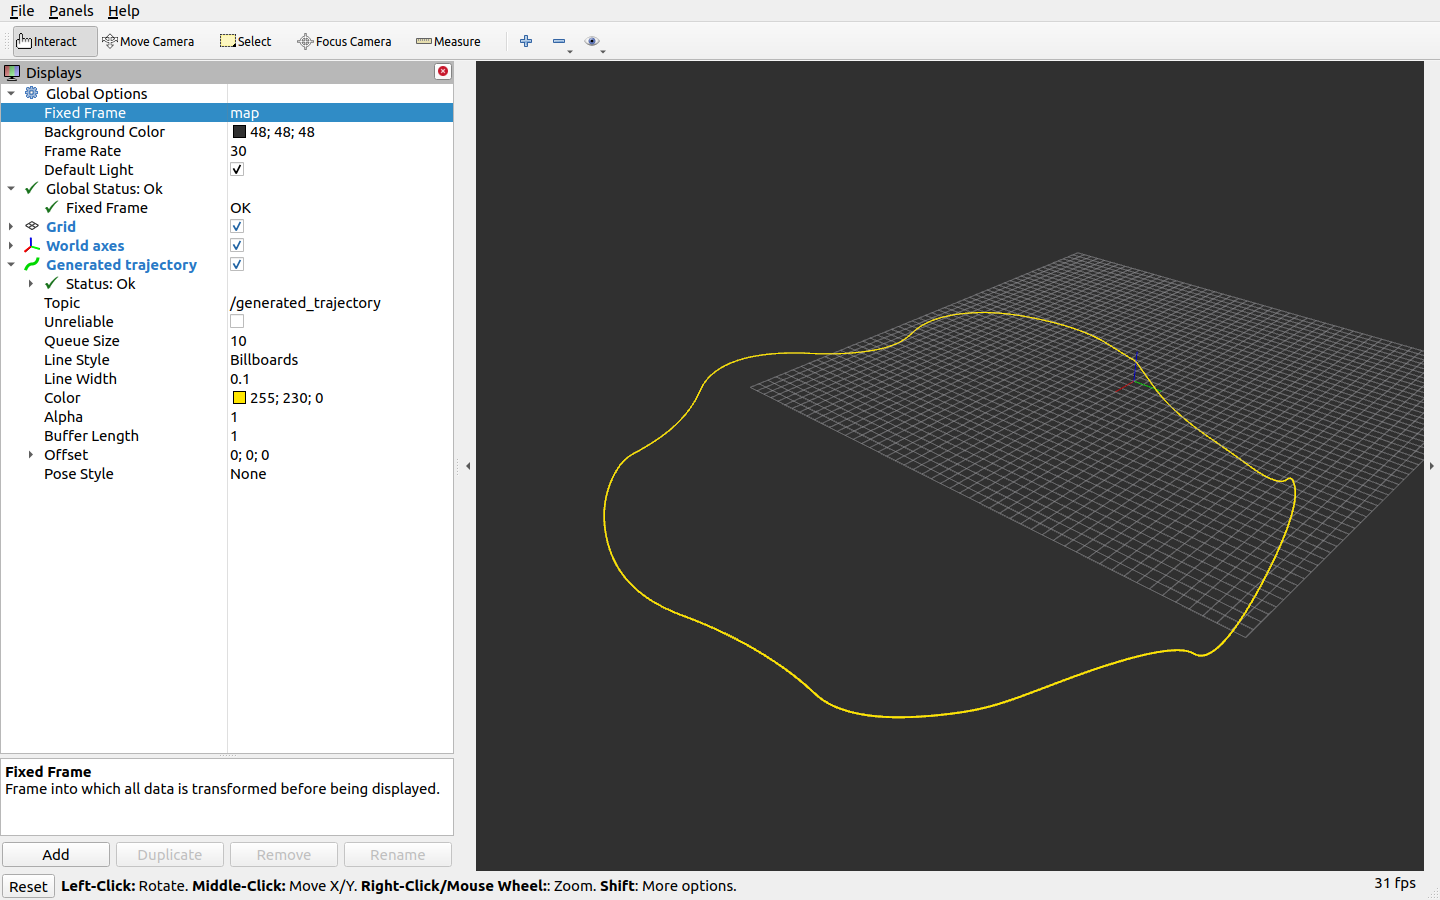
\includegraphics[width=0.95\textwidth]{figures/test-pm-rviz-result.png}
\caption[轨迹可视化结果]{重构轨迹的可视化结果。}
\end{figure}

下图由同次运行保存的 363 个位置样本生成，左侧显示三维重构轨迹与按上述公式生成的航点标记，并标注起始点与第七个圆形航点的重合关系；右侧显示按上述时间轴排列的\(x(t)\)、\(y(t)\)、\(z(t)\)位置曲线。实际位置样本的 z 坐标约为\(-0.6082\text{ m}\)至\(4.6077\text{ m}\)，说明固定高度的航点并不意味着航点之间的重构轨迹保持固定高度：本示例采用具有非零 z 分量的参考运动方向，各解析航段在连接这些航点时产生了高度变化。该位置数据仅包含轨迹的位置分量，图中未将速度或加速度作为输出，也未用位置差分构造这些量。

\begin{figure}[H]
\centering
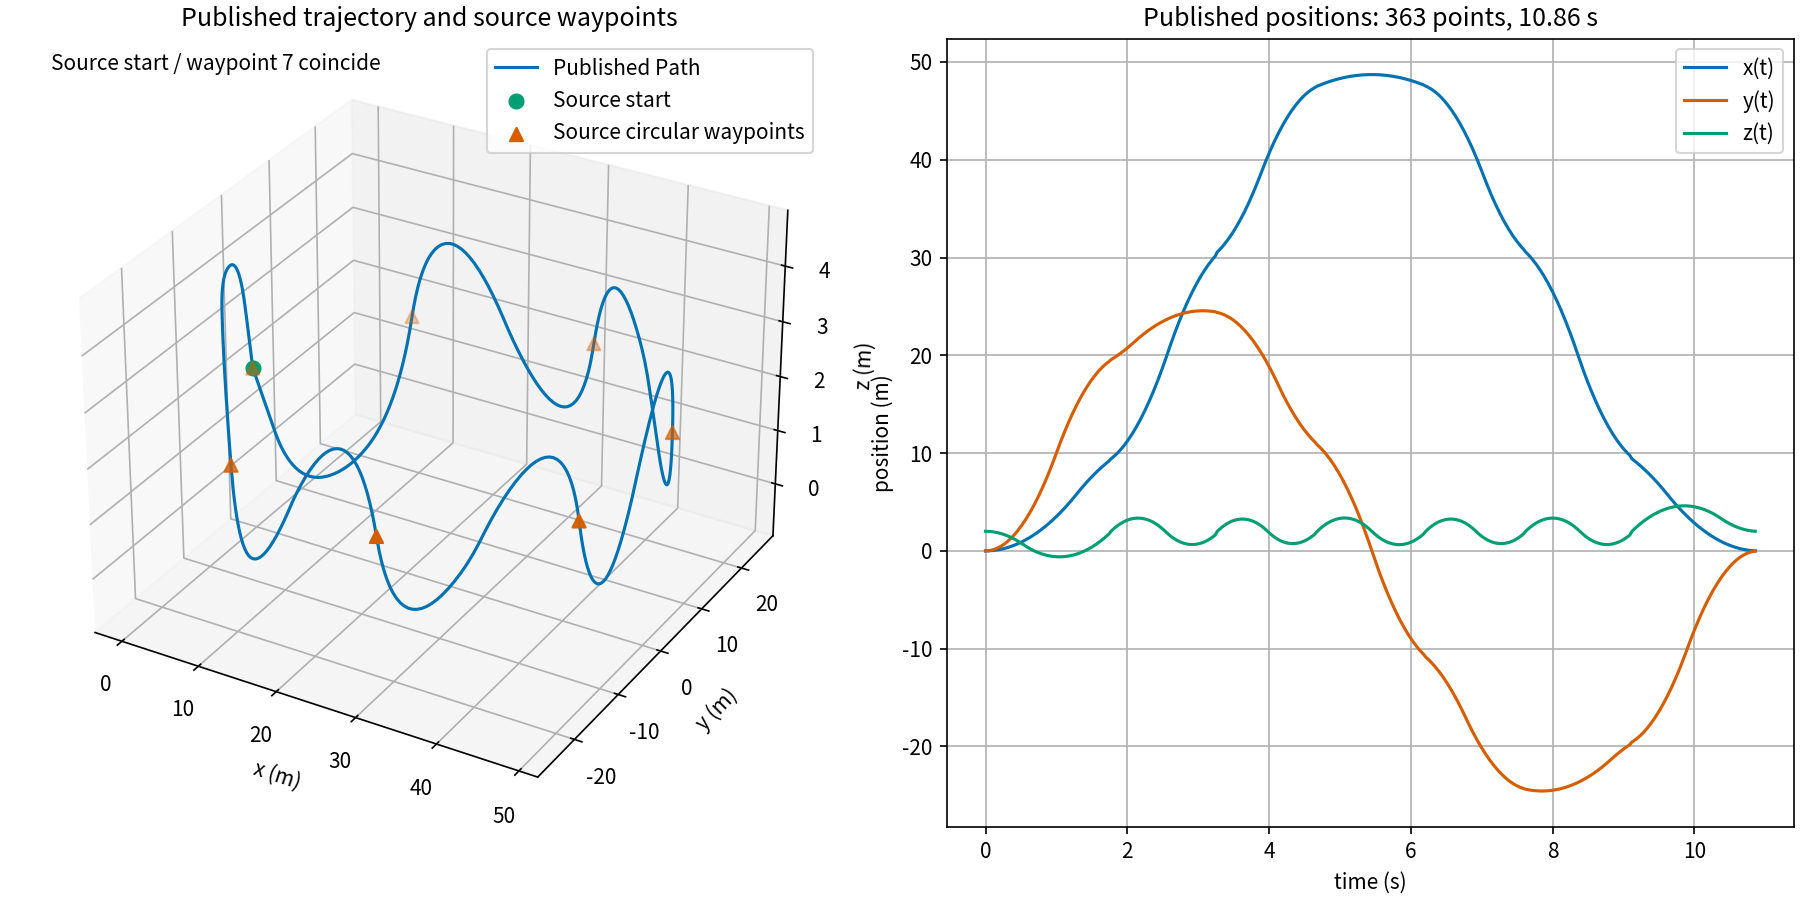
\includegraphics[width=0.95\textwidth]{figures/test-pm-trajectory-curves.png}
\caption[重构轨迹的位置数据曲线]{同次运行的三维位置轨迹、圆形航点及位置分量曲线。}
\end{figure}

上述实际计算展示了从航点与初始状态输入、质点轨迹求解和解析采样，到位置序列整理及可视化的处理过程。记录的计算耗时、位置样本数量及空间变化仅对应本示例配置；本次结果未提供与其他方法的对照数据，因而不据此推导计算速度提升比例或其他未测量的性能增益。

\section{算法增益效果}

与按距离比例或固定速度直接分配航段时间的方式相比，本发明显式利用每一坐标轴的正、负加速度边界以及航段两端速度，通过两阶段恒加速度模型计算候选转移时间。因此，所得时间分配能够反映速度变化和轴向位移对航段执行难度的共同影响，而不是仅由几何长度决定。

本发明将三个坐标轴分别表示为低维分段恒加速度问题，以独立最短时间的最大值作为严格下界，再以三轴共同可行性决定真正的航段公共时间。该机制避免三个轴按各自时间独立到达造成三维航点失配，也避免把未经验证的最大轴时间误作可执行边权。每条有效边在进入图搜索前即具有满足端点状态和加速度边界的同步参数。

本发明利用参考运动方向约束候选速度方向，只对速度幅值进行离散采样。在每个中间航点设置\(K\)个候选速度时，节点数量随航点数近似线性增长，相邻层边数为前后层候选数乘积。与对三个速度分量分别设置\(K\)个候选值所产生的\(K^3\)个速度向量相比，方向约束能够明显降低中间速度候选空间的维度，并减少与参考路径局部走向显著冲突的候选速度。

本发明不是逐段贪心地选择局部最短时间。由于同一个中间航点速度同时决定前一航段的末速度和后一航段的初速度，分层速度图以累计时间为目标进行跨航段选择。图结构只向下一航点层连接且不含循环，逐层动态规划会比较每个后级节点的全部前驱，从而在固定有限候选图中得到累计公共时间最小的速度组合。

本发明在计算候选边时完成共同时间验证，并在松弛成功时把前驱节点和该边的可行参数一并保存；搜索结束后只需对回溯所得边进行解析采样，无需为未入选边生成密集轨迹，也无需用另一套方程重新求解参数。分段恒加速度解析式直接给出位置、速度和加速度，位置与速度在阶段切换处连续，适合用作二阶积分对象的参考输入。

本发明的输入只要求有序航点及参考运动方向，不限定航点来自何种规划算法。输入可以由人工设定、地图搜索、采样规划、曲线离散或者已有轨迹抽取得到。因此，本发明能够作为独立的时间重分配后处理模块，与不同前端规划方案组合使用，并且不会把前端规划器的具体实现引入本发明的必要技术特征。

本发明能够分别设置三个坐标轴的加速度上下界，并能够处理不对称边界、零位移轴和方程退化情况。通过可行根筛选、缩放因子检查和不可行边标记，可以避免将不满足预设运动边界的候选转移纳入最短路径。候选速度数量、采样间隔和输出周期均可按计算资源和轨迹精度需要配置。

应当说明，本发明的直接效果是实现航点序列上的时间重分配和质点状态重构。本发明不以能耗最小、高阶导数连续或者完整刚体动力学最优作为必要效果。若输入仅包含稀疏航点而未附带安全走廊约束，重构曲线在航点之间可能不同于输入曲线，因而可在具体系统中附加碰撞复核或安全走廊约束，但该附加处理不改变本发明的核心时间重分配机制。

\end{document}
